%% 
%%	This is file 'beamer_sample.tex'
%%	according to an MPIDR's PowerPoint template (?)
%%	
%%	by Eric Naujoks
%%
%%	Problems, bugs and comments to 
%%	naujoks@demogr.mpg.de
%%

%%%%%%%%%%%%%%%%%%%%%%%%%%%%%%%%%%
%%	Praelegomena								%%
%%%%%%%%%%%%%%%%%%%%%%%%%%%%%%%%%%
%%	- Make sure that you use utf8-encoding for all your .tex-files!!! (TeXnicCenter since version 2.0)
%%	- TeXnicCenter update: MPIDR intranet > Hard- & Sortfware > Software > Script and text editors > TeXnicCenter

\documentclass[20pt]{beamer}

\usepackage[ngerman,english]{babel}
\usepackage{tikz}
\usepackage[normalem]{ulem}
\geometry{paperwidth=10in, paperheight=7.5in}
\usepackage{animate}

\usepackage[utf8]{inputenc}

\usepackage[mpidr]{./mpidr/beamerthemeMPIDR}
\usefonttheme{serif}


%% Declaring title and author
\title{Properties of generalized Lexis identities}
\subtitle{Tim Riffe \\ Jonas Sch{\"o}ley}		%%

%%	the institute's logo
\renewcommand{\mylogo}{\includegraphics[width=4.7in]{mpidr_logo_colour_en}}
\usepackage{color}
\definecolor{mygray}{rgb}{0.8,0.8,0.8}

\defbeamertemplate{description item}{align left}{\insertdescriptionitem\hfill}
%%	should be the very last package to be loaded
\usepackage{hyperref}

%%%%%%%%%%%%%%%%%%%%%%%%%%%%%%%%%%
%%	Beginning of the document		%%
%%%%%%%%%%%%%%%%%%%%%%%%%%%%%%%%%%
\begin{document}

%%	titlepage - fixed frame:
%%	========================

\begin{frame}
	\titlepage
\end{frame}
%-------------------
\begin{frame}[plain]
\begin{block}{Objective}
We describe the construction and reflect on the composition and identification
of higher order temporal identities.
\end{block}

\end{frame}
%-------------------

%-------------------

\begin{frame}[plain]
\makebox[\linewidth]{\includegraphics[width=\paperwidth]{Figures/LexisSimple.JPG}}
\end{frame}

%-------------------

\begin{frame}[plain]
\makebox[\linewidth]{\includegraphics[width=\paperwidth]{Figures/LexisSimple2.png}}
\end{frame}

%-------------------

\begin{frame}[plain]
\begin{block}{APC identity}
P -- C = A
\end{block}
\only<1>{\includegraphics[width=23cm]{Figures/APCtimeline.JPG}}
\only<2>{\includegraphics[width=23cm]{Figures/APCtimeline2.png}}
\only<3>{\includegraphics[width=23cm]{Figures/APCtimeline3.png}}
\end{frame}

%-------------------

\begin{frame}[plain]
\Large
Events and durations are key.
\end{frame}

%-------------------

\begin{frame}[plain]
\Large
Events may be anchored or scale\\
Durations may be either scaling or fixed\\
Scaling time measures move along a lifeline, whereas anchored events and fixed
durations are lifelong attributes.
\end{frame}


%-------------------

\begin{frame}[plain]
\begin{center}
\only<1>{\includegraphics[height=18cm]{Figures/APCTri.JPG}}
\only<2>{\includegraphics[height=18cm]{Figures/APCTri2.png}}
\end{center}
\end{frame}

%-------------------

\begin{frame}[plain]
\begin{center}
\Large Some categories
\begin{itemize}[<+->]
  \item C is an anchored event
  \item P scales over a lifeline
  \item but any given P is anchored, so it's like an event.
  \item A is a function of P, so it scales along lifelines too.
\end{itemize}
\end{center}
\end{frame}

%-------------------

\begin{frame}[plain]
\begin{block}{Dimensionality}
APC is based on 2 events. Its tesselated diagram is 2d. hmmm
\end{block}
\begin{center}
\includegraphics[height=15cm]{Figures/APCTri2.png}
\end{center}
\end{frame}

%-------------------

\begin{frame}[plain]
\begin{center}
\Large What happens if we add another event?\\ \vspace{1em}
such as \emph{death}.
\end{center}
\end{frame}

%-------------------

\begin{frame}[plain]
\begin{block}{APCTDL identity}
1) \{P -- C = A\}  ,  2) \{D -- P = T  \} , 3) \{D -- C = L\}
\end{block}
\begin{center}
\includegraphics[width=23cm]{Figures/CPDtimeline.jpeg}
\end{center}
\end{frame}

%-------------------

\begin{frame}[plain]
\begin{center}
\only<1>{\includegraphics[height=15cm]{Figures/apctdltetra.jpg}}
\only<2>{\includegraphics[height=15cm]{Figures/apctdltetra2.png}}
\end{center}
\end{frame}

%-------------------

\begin{frame}[plain]
\begin{block}{Dimensionality}
APCTDL has 3 events. Its extent after tesselation is 3d. hmmm
\end{block}
\vspace{1em}
\begin{center}
\includegraphics[scale=2]{Figures/contemporary-decorative-objects-and-figurines.jpg}

a nice wooden tetrahedron
\end{center}
\end{frame}

%-------------------

\begin{frame}[plain]
\begin{center}
\Large Further considerations
\begin{itemize}[<+->]
  \item $n$ events implies $n$-dimensionality
  \item 3 events implies 3 durations.
  \item in general $n$ events implies $\binom{n}{2}$ durations.
\end{itemize}
\end{center}
\end{frame}

%-------------------

\begin{frame}[plain]
\begin{center}
\Large $n$ events implies $\binom{n}{2}$ durations

\only<1>{\vspace{1em}\includegraphics[height=7cm]{Figures/Gp2.jpeg} ~
\includegraphics[height=7cm]{Figures/Gp3.jpeg} ~
\includegraphics[height=7cm]{Figures/Gp4.jpeg}  

~~
}
\only<2>{\vspace{1em}\includegraphics[height=7cm]{Figures/Gp22.png} ~
\includegraphics[height=7cm]{Figures/Gp32.png} ~
\includegraphics[height=7cm]{Figures/Gp42.png} 

(Just complete the graph by connecting all ends)
}

\end{center}
\end{frame}

%-------------------

\begin{frame}[plain]
\begin{center}
\Large
\begin{itemize}[<+->]
  \item $n$ events imply $\binom{n}{2}$ durations
  \item $n$ events imply an identity of $n + \binom{n}{2}$ time measures
  \item This identity can be represented by a complete graph on $n+1$ vertices,
  say $G^n$.
  \item $G^n$ may have subidentities.
\end{itemize}

\end{center}
\end{frame}

%-------------------

\begin{frame}[plain]
\begin{center}
\Large
\includegraphics[height=7cm]{Figures/Gp32.png} ~
\includegraphics[height=7cm]{Figures/Gp42.png} 
\begin{itemize}[<+->]
  \item $\binom{n}{2}$ subidentities consist in two events plus a duration
  \item $\binom{n}{3}$ subidentities consist in 3 durations only
  \item There are $\binom{n+1}{n'+1}$ subidentities of dimension $n'$ in general
\end{itemize}

\end{center}

\end{frame}

% -----------------

\begin{frame}[plain]
% something on classes of subidentities
\Large

\begin{center}
\only<1>{\includegraphics[height=12cm]{Figures/Composition.png}}
\only<2>{\includegraphics[height=12cm]{Figures/Composition1.png}}
\only<3>{\includegraphics[height=12cm]{Figures/Composition2.png}}
\only<4>{\includegraphics[height=12cm]{Figures/Composition3.png}}

A 4-event identity
\end{center}

\end{frame}

% -----------------

\begin{frame}[plain]
% something on classes of subidentities
\Large

\begin{center}
\includegraphics[height=8cm]{Figures/Composition3.png}
\end{center}
\begin{itemize}[<+->]
  \item $\binom{n}{2}$ triads of 2 events and 1 duration
  \item of which $\binom{n-1}{2}$ are 2 anchored events and 1 fixed duration
  \item and $n-1$ are 1 anchored event, period, and 1 scaling duration.
  \item $\binom{n}{2} = \binom{n-1}{2} + (n-1)$
\end{itemize}
\end{frame}

% -----------------

\begin{frame}[plain]
% something on classes of subidentities
\Large

\begin{center}
\includegraphics[height=8cm]{Figures/Composition3.png}
\end{center}
\begin{itemize}[<+->]
  \item $\binom{n}{3}$ triads of 3 durations
  \item of which $\binom{n-1}{3}$ are 3 fixed
  durations
  \item and $\binom{n-1}{2}$ are of 2 scaling and 1 fixed duration
  \item $\binom{n}{3} = \binom{n-1}{3} + \binom{n-1}{2}$
\end{itemize}
\end{frame}

% -----------------

\begin{frame}[plain]
% something on classes of subidentities

\begin{center}
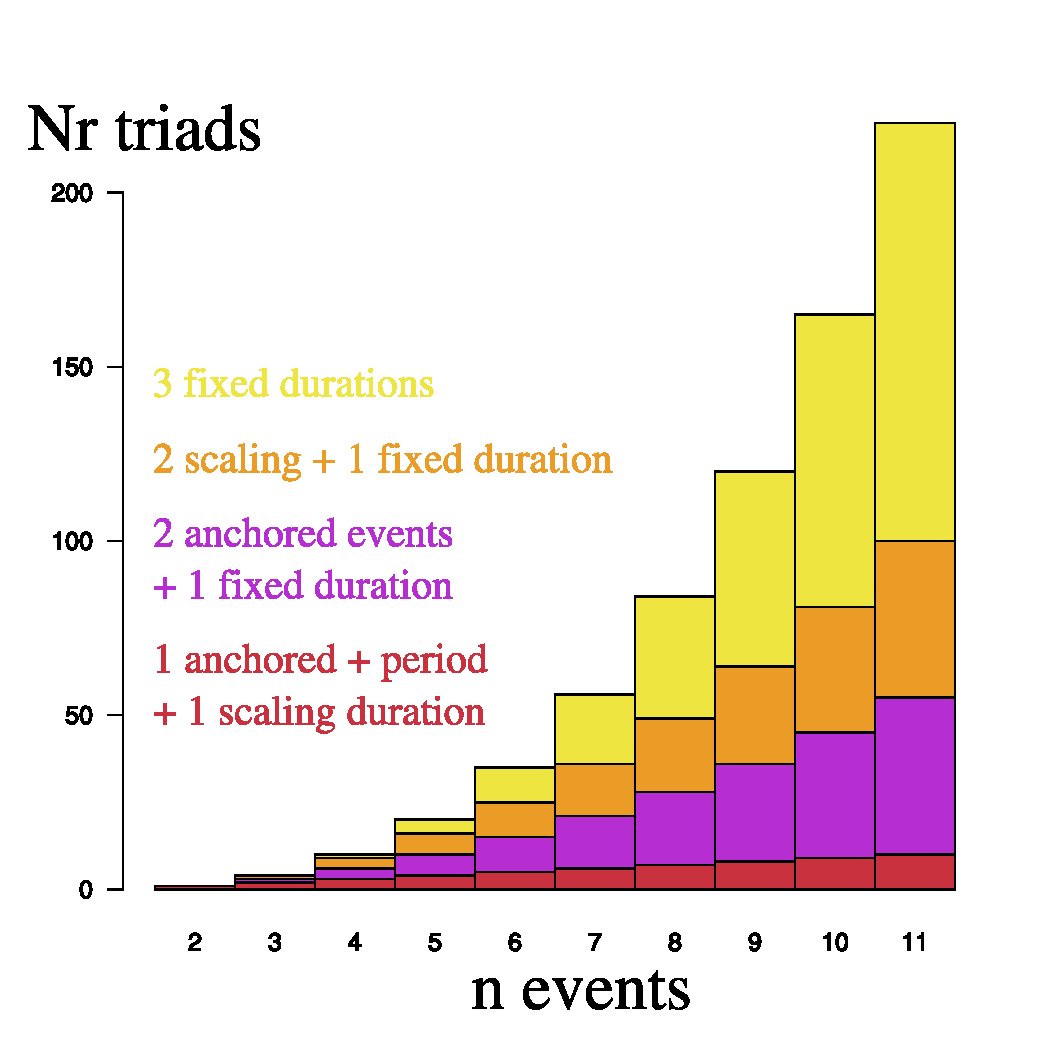
\includegraphics[scale=1]{Figures/id3compmarked.pdf}
\end{center}

\end{frame}

% -----------------

\begin{frame}[plain]
% something on classes of subidentities
\Large

\begin{block}{Identifiability}
Given an id from $n$ events, there are $(n+1)^{(n-1)}$ potential sets of $n$
time measures (events and/or durations) whose linear combination yields the full
implied identity. These can be represented as the minimal spanning trees (MST)
of $G^n$.
\end{block}

\end{frame}

\begin{frame}

\begin{center}
\includegraphics[height = .8\textheight]{Figures/sorting-hat-spider.jpg}
\end{center}

``Sorting Hat'' Spider (Eriovixia gryffindori). Location: India\\
HT \url{http://earthsky.org}
\end{frame}
%%%%%%%%%%%%%%%%%%%%%%%%%%%%%%%%%%
%%	End of the document			%%
%%%%%%%%%%%%%%%%%%%%%%%%%%%%%%%%%%
\end{document}










